% !TeX spellcheck = fr_FR
\chapter{Chapitre 7 : Base de données et données persistantes}

\section*{Pourquoi un chapitre sur la base de données ?}

Cette application est construite autour d'un \textit{graphe spatial} de points d'arrêt. Le rendu cartographique en temps réel, l'analyse des problèmes et la consolidation des correspondances s'appuient sur un schéma de base de données optimisé pour la lecture, avec une logique d'\textit{ingestion} explicite. 

Ce chapitre rend cette mécanique visible, avec des extraits de code et schémas.

\vspace{0.5em}
Le chapitre \texttt{chap8.tex} plongera ensuite dans le backend (API, endpoints, sécurité, pagination, etc.), en s'appuyant sur les éléments que nous posons ici.

\subsection*{Essentiels à retenir}
\begin{itemize}
  \item \textbf{Ligne auto-suffisante pour la carte} : une ligne \texttt{stops} suffit pour dessiner un marqueur (ATLAS ou OSM) \Rightarrow pas de \texttt{JOIN} au scroll.
  \item \textbf{Fenêtre cartographique SARGable} : index \texttt{atlas\_lat/lon} \& \texttt{osm\_lat/lon} \Rightarrow filtrage par bbox très sélectif.
  \item \textbf{Détails séparés} : \texttt{atlas\_stops} et \texttt{osm\_nodes} servent les popups à la demande (\textit{lazy}).
  \item \textbf{Persistance durable} : \texttt{persistent\_data} stocke solutions/notes qui \og survivent \fg{} aux ré-imports et sont réappliquées.
  \item \textbf{Séparation Auth} : schéma \texttt{auth\_db} isolé via \texttt{SQLAlchemy binds} (sécurité, gouvernance des droits ; détail au Chap.~\ref{chap:auth}).
\end{itemize}

\section{Importer les données: le rôle de \texttt{import\_data\_db.py}}
L'import est orchestré par le script \texttt{import\_data\_db.py}. Il nettoie, croise des sources, calcule des priorités de problèmes, et construit des artefacts prêts pour l'interface.

\subsection*{Vue d'ensemble}
\begin{codebox}[language=Python]{Pipeline d'import des données}
build_route_direction_mapping()  # cartographie GTFS/OSM/HRDF -> (route, direction) <-> (noeuds, SLOIDs)
load_route_data()                # routes par SLOID (ATLAS) et par node_id (OSM)
load_unified_route_data()        # vue unifiée (gtfs/hrdf) par SLOID
import_to_database(...)          # insère stops, détails ATLAS/OSM, routes, problèmes
apply_persistent_solutions()     # réapplique les solutions/notes persistantes
\end{codebox}

L'import crée des \textit{stops} de trois types:\ \texttt{matched} (paires ATLAS–OSM), \texttt{unmatched} (ATLAS isolé), \texttt{osm} (OSM isolé). Ces valeurs de \texttt{stop\_type} sont appliquées par logique métier lors de l'import et peuvent être modifiées via match manuel. Les détails riches (ex: opérateur ATLAS, tags OSM, routes) sont stockés dans des tables dédiées.

Pour la ré-application des données persistantes, le script balaye la table \texttt{persistent\_data} et met à jour les nouveaux enregistrements:

\begin{codebox}[language=Python]{Ré-application des solutions persistantes}
# Extrait de import_data_db.py -> apply_persistent_solutions()
persistent_solutions = session.query(PersistentData)\
    .filter(PersistentData.note_type.is_(None)).all()

for ps in persistent_solutions:
    matching_stops = session.query(Stop)\
        .filter((Stop.sloid == ps.sloid) | (Stop.osm_node_id == ps.osm_node_id))\
        .all()
    
    for stop in matching_stops:
        problem = session.query(Problem).filter(
            Problem.stop_id == stop.id,
            Problem.problem_type == ps.problem_type
        ).first()
        
        if problem:
            problem.solution = ps.solution
            problem.is_persistent = True
\end{codebox}

\section{Schéma logique: les tables qui comptent}

Le schéma applicatif est défini dans \texttt{backend/models.py} et utilise l'ORM SQLAlchemy\citeref{ref:sqlalchemy_docs} pour interagir avec la base de données. Voici les entités principales:

\begin{description}
  \item[\texttt{stops}] Table centrale pour le rendu cartographique. Colonnes clefs: \texttt{sloid}, \texttt{stop\_type}, \texttt{match\_type}, coordonnées (\texttt{atlas\_lat/lon} et \texttt{osm\_lat/lon}), \texttt{distance\_m}, \texttt{osm\_node\_type}, \texttt{atlas\_duplicate\_sloid}.
  
  \item[\texttt{atlas\_stops}] Détails ATLAS par \texttt{sloid}: désignation, opérateur, routes unifiées, notes persistantes.
  
  \item[\texttt{osm\_nodes}] Détails OSM par \texttt{osm\_node\_id}: tags de transport, opérateur, routes OSM, notes.
  
  \item[\texttt{problems}] Détections automatiques (\texttt{distance}, \texttt{unmatched}, \texttt{attributes}, \texttt{duplicates}), solution éventuelle, \texttt{priority} et traçabilité auteur.
  
  \item[\texttt{persistent\_data}] Stockage des solutions et notes destinées à survivre aux ré-imports.
  
  \item[\texttt{routes\_and\_directions}] Consolidation GTFS/HRDF/OSM avec clés multiples: (\texttt{route\_id}, \texttt{direction\_id}) pour GTFS/OSM et (\texttt{line\_name}, \texttt{direction\_uic}) pour HRDF, plus \texttt{route\_id\_normalized} pour unification.
\end{description}

\paragraph{Note sur l'authentification} Un schéma séparé (\texttt{auth\_db}) stocke les utilisateurs (\texttt{users}) et les événements (\texttt{auth\_events}) via un bind SQLAlchemy distinct (\texttt{\_\_bind\_key\_='auth'}). Il est volontairement isolé du schéma métier; nous le détaillons au Chap.~\ref{chap:auth}.

\subsection*{Diagramme conceptuel}

\begin{figure}[H]
  \centering
  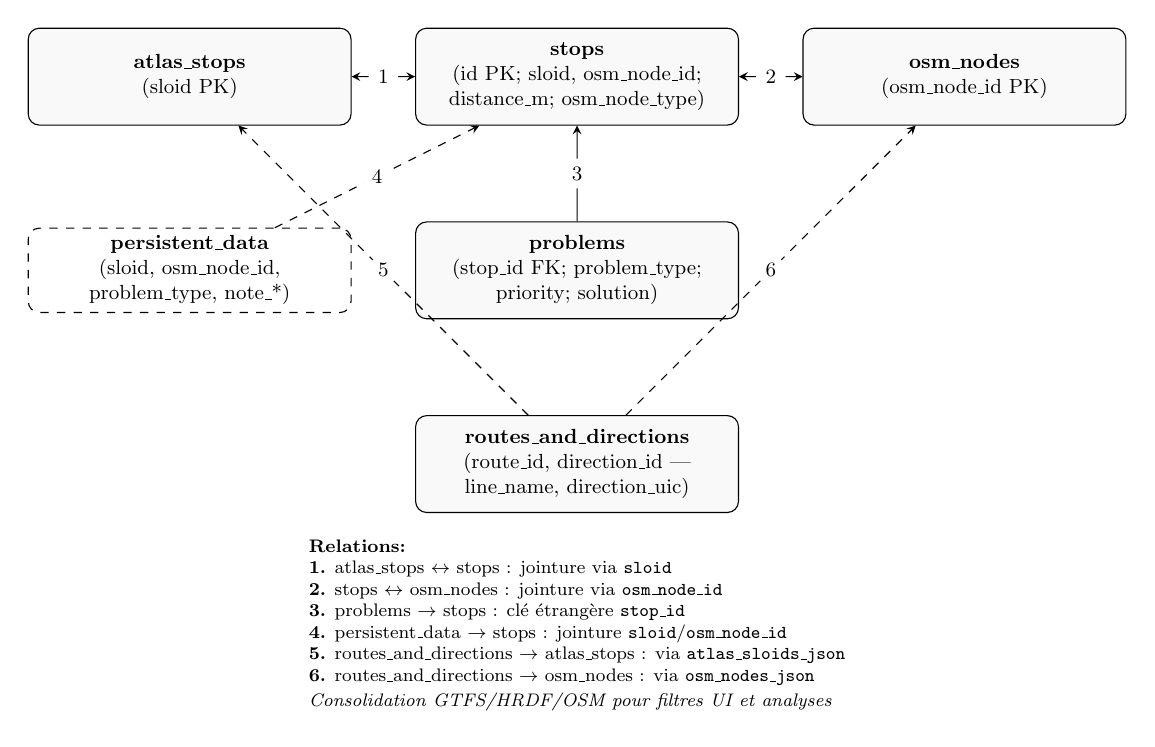
\begin{tikzpicture}[>=stealth, scale=0.82, transform shape]
    \tikzstyle{tbl}=[draw, rounded corners, minimum width=5cm, minimum height=1.5cm, align=center, fill=gray!5, font=\small]
    \tikzstyle{ghost}=[draw, dashed, rounded corners, minimum width=5cm, minimum height=1.3cm, align=center, font=\small]

    % Utilisation de coordonnées absolues pour un meilleur contrôle
    % Ligne supérieure: atlas_stops - stops - osm_nodes
    \node[tbl] (atlas) at (0,3) {\textbf{atlas\_stops}\\ (sloid PK)};
    \node[tbl] (stops) at (6,3) {\textbf{stops}\\ (id PK; sloid, osm\_node\_id;\\ distance\_m; osm\_node\_type)};
    \node[tbl] (osm) at (12,3) {\textbf{osm\_nodes}\\ (osm\_node\_id PK)};
    
    % Ligne médiane: persistent_data - problems
    \node[ghost] (persist) at (0,0) {\textbf{persistent\_data}\\ (sloid, osm\_node\_id,\\ problem\_type, note\_*)};
    \node[tbl] (problems) at (6,0) {\textbf{problems}\\ (stop\_id FK; problem\_type;\\ priority; solution)};
    
    % Ligne inférieure: routes_and_directions (centré)
    \node[tbl] (routes) at (6,-3) {\textbf{routes\_and\_directions}\\ (route\_id, direction\_id |\\ line\_name, direction\_uic)};

    % Relations avec numéros
    \draw[<->] (atlas) -- node[fill=white, circle, inner sep=2pt]{\small 1} (stops);
    \draw[<->] (stops) -- node[fill=white, circle, inner sep=2pt]{\small 2} (osm);
    \draw[->] (problems) -- node[fill=white, circle, inner sep=2pt]{\small 3} (stops);
    \draw[dashed,->] (persist) -- node[fill=white, circle, inner sep=2pt]{\small 4} (stops);
    \draw[dashed,->] (routes) -- node[fill=white, circle, inner sep=2pt]{\small 5} (atlas);
    \draw[dashed,->] (routes) -- node[fill=white, circle, inner sep=2pt]{\small 6} (osm);

    % Légende des relations
    \node[below of=routes, node distance=2.5cm, align=left, font=\footnotesize] (legend) {
      \textbf{Relations:}\\
      \textbf{1.} atlas\_stops $\leftrightarrow$ stops : jointure via \texttt{sloid}\\
      \textbf{2.} stops $\leftrightarrow$ osm\_nodes : jointure via \texttt{osm\_node\_id}\\
      \textbf{3.} problems $\rightarrow$ stops : clé étrangère \texttt{stop\_id}\\
      \textbf{4.} persistent\_data $\rightarrow$ stops : jointure \texttt{sloid}/\texttt{osm\_node\_id}\\
      \textbf{5.} routes\_and\_directions $\rightarrow$ atlas\_stops : via \texttt{atlas\_sloids\_json}\\
      \textbf{6.} routes\_and\_directions $\rightarrow$ osm\_nodes : via \texttt{osm\_nodes\_json}\\[0.2em]
      \textit{Consolidation GTFS/HRDF/OSM pour filtres UI et analyses}
    };
  \end{tikzpicture}
  \caption{Schéma relationnel des tables principales (liens via champs de jointure; FK explicite seulement pour \texttt{problems.stop\_id}).}
\end{figure}

\noindent
Remarque: les liens \og stops $\rightarrow$ détails \fg{} sont réalisés par \textit{jointures explicites} (\texttt{sloid}, \texttt{osm\_node\_id}) plutôt que des clés étrangères rigides. Ce choix facilite l'ingestion et limite les verrouillages lors des rafraîchissements, tout en gardant des \textit{indexes} ciblés pour les requêtes critiques. L'ORM SQLAlchemy définit des relations \texttt{lazy='joined'} sur ces champs pour optimiser les accès.

\subsection*{Index utiles pour la carte}
\begin{itemize}
  \item \texttt{idx\_atlas\_lat\_lon} et \texttt{idx\_osm\_lat\_lon} pour filtrer vite par fenêtre cartographique.
  \item \texttt{idx\_stop\_type\_match\_type} pour les filtres dynamiques.
  \item \texttt{idx\_distance\_m} pour les tris par distance.
  \item Sur \texttt{routes\_and\_directions}: \texttt{idx\_osm\_route\_direction}, \texttt{idx\_atlas\_route\_direction}, \texttt{idx\_atlas\_line\_direction\_uic}, et \texttt{idx\_source} (colonne \texttt{source} pour différencier GTFS/HRDF). Le champ \texttt{route\_id\_normalized} sert à l'unification cross-sources.
\end{itemize}

\section{Pros et cons du schéma vis-à-vis du rendu cartographique}
\subsection*{Points forts}
\begin{itemize}
  \item \textbf{Lecture optimisée}: une ligne de \texttt{stops} suffit pour dessiner un marqueur (ATLAS ou OSM) sans \texttt{JOIN}.
  \item \textbf{SARGable viewport}: la requête de fenêtre cartographique est \emph{sélective} grâce aux index lat/lon des deux mondes (extrait d'API ci-dessous).
  \item \textbf{Détails séparés}: les tables \texttt{atlas\_stops} et \texttt{osm\_nodes} chargent les popups à la demande (lazy) sans gonfler la ligne \texttt{stops}.
  \item \textbf{Routes consolidées}: la table \texttt{routes\_and\_directions} alimente les filtres par ligne et direction côté UI.
\end{itemize}

\subsection*{Compromis}
\begin{itemize}
  \item \textbf{Intégrité logique}: l'absence de FK strictes suppose une discipline d'import (gérée par \texttt{import\_data\_db.py}).
  \item \textbf{Duplication contrôlée}: certaines valeurs (ex: \texttt{distance\_m}) sont redondantes par design pour éviter des calculs à la volée.
  \item \textbf{Évolution des tags OSM}: les champs \texttt{osm\_*} sont \textit{snapshottés}; toute évolution nécessite un nouvel import.
\end{itemize}

\subsection*{La requête de fenêtre}

\begin{codebox}[language=Python]{Filtrage géographique optimisé — backend/blueprints/data.py}
# Requête SARGable pour l'endpoint /api/data
viewport_sargable = or_(
    # Points ATLAS dans la fenêtre
    and_(Stop.atlas_lat.between(min_lat, max_lat),
         Stop.atlas_lon.between(min_lon, max_lon)),
    
    # Points OSM seuls dans la fenêtre  
    and_(Stop.atlas_lat.is_(None), Stop.atlas_lon.is_(None),
         Stop.osm_lat.between(min_lat, max_lat),
         Stop.osm_lon.between(min_lon, max_lon))
)

query = query.filter(viewport_sargable)
\end{codebox}


\section{Données persistantes: comment elles survivent aux ré-imports}
Le mécanisme de persistance se trouve à deux endroits:\ (i) l'API de gestion (\texttt{/api/make\_solution\_persistent}, \texttt{/api/save\_note/...}),\ (ii) l'étape \texttt{apply\_persistent\_solutions()} de l'import.

\subsection*{Côté base}
La table \texttt{persistent\_data} stocke:
\begin{itemize}
  \item des \textbf{solutions} par triplet \texttt{(sloid, osm\_node\_id, problem\_type)};
  \item des \textbf{notes} persistantes côté ATLAS (\texttt{note\_type = 'atlas'}) ou OSM (\texttt{'osm'}).
\end{itemize}

\subsection*{Côté web (UI)}
Dans l'interface \og Problèmes \fg{}, l'utilisateur peut:
\begin{itemize}
  \item résoudre un problème, puis \textit{rendre la solution persistante} (bouton dédié) ;
  \item saisir une note côté ATLAS ou OSM et la marquer persistante ;
  \item effectuer un \textit{match manuel} entre deux entrées (ATLAS $\leftrightarrow$ OSM) et l'enregistrer de manière durable.
\end{itemize}
Nous ajouterons des captures d'écran de l'interface dans une version ultérieure du manuscrit.

\subsection*{Un mini-exemple côté navigateur}

\begin{codebox}{Match manuel persistant — interface web}
// Extrait simplifié de la logique JS de match manuel
$.ajax({
    url: '/api/manual_match',
    method: 'POST',
    contentType: 'application/json',
    data: JSON.stringify({
        atlas_stop_id: atlasId,
        osm_stop_id: osmId,
        make_persistent: true
    }),
    success: function(response) {
        console.log('Match persistant créé:', response);
    }
});
\end{codebox}

\noindent
Lors du prochain import, la solution manuelle réapparaîtra \textit{sans effort} grâce à \texttt{apply\_persistent\_solutions()}.

\section{Performance: pourquoi ça défile vite sur la carte}

L'expérience utilisateur fluide de la carte interactive repose sur deux ingrédients architecturaux clés:

\begin{description}
  \item[Ligne auto-suffisante pour le rendu] La table \texttt{stops} contient toutes les informations nécessaires au rendu d'un marqueur. Un \textit{viewport query} n'a pas besoin de joindre des tables lourdes: la position et la nature du marqueur (\texttt{osm\_node\_type}) sont \og en main \fg{}.
  
  \item[Index spatiaux ciblés] Les clauses \texttt{BETWEEN} sur les coordonnées (\texttt{atlas\_lat/lon}, \texttt{osm\_lat/lon}) exploitent des index dédiés, permettant une sélection très rapide par fenêtre géographique.
\end{description}

\paragraph{Chargement différé des détails} Les informations riches (opérateur, routes, notes) sont chargées \textit{au clic} pour construire les popups — ce qui évite de surcharger la phase de \textit{fetch} initial. Cette stratégie de \textit{lazy loading} maintient des temps de réponse constants même avec des milliers de points.

\paragraph{Optimisations côté client} Les marqueurs qui se superposent géographiquement sont \og décalés \fg{} de quelques pixels afin de rester individuellement cliquables, sans impact sur les performances de rendu.



